\section{Results}


The STEM-DPC vector maps in Figure \ref{fig:STEM-DPC} reveal that the majority of the polygons exhibit magnetization forming closed loops in the plane of the specimen. These vortex-like configurations are clearly visible as a continuous rotation of the magnetization vectors around the center of each structure. One can observe that polygons with successful intersections, or vortices, between all magnetic domains exhibit a high curl within these vortices, indicated by a bright spot in Figure \ref{fig:hexagon}.
\begin{figure}[H]
    \centering
    \includegraphics[width=\columnwidth]{Images/Stem_DPC_high_contrast.png}
    \caption{STEM-DPC overview image. %with white outlines surrounding analyzed figures of interest
    }
    \label{fig:STEM-DPC}
\end{figure}
\vspace{-1cm}
The tendency to form discrete magnetic domains varies with polygon geometry. In polygons with fewer sides (e.g. triangles and squares), the magnetization shows clear angular discontinuities aligned with the polygon edges. In contrast, polygons with a larger number of sides (e.g. octagons and nonagons) have smoother rotational fields that better resemble circular vortex states.

%the average curl drops sharply between the hexagon and heptagon.

The analysis of curl flux as a function of number of sides revealed a linear or decaying exponential trend for all three sets of polygons. Where the increasing number of sides resulted in a lower curl per area, though with the triangles excluded due to mismatch with the rest of the polygons. The reason for this mismatch is too be discussed in later sections.   

\begin{figure}[H]
    \centering  
    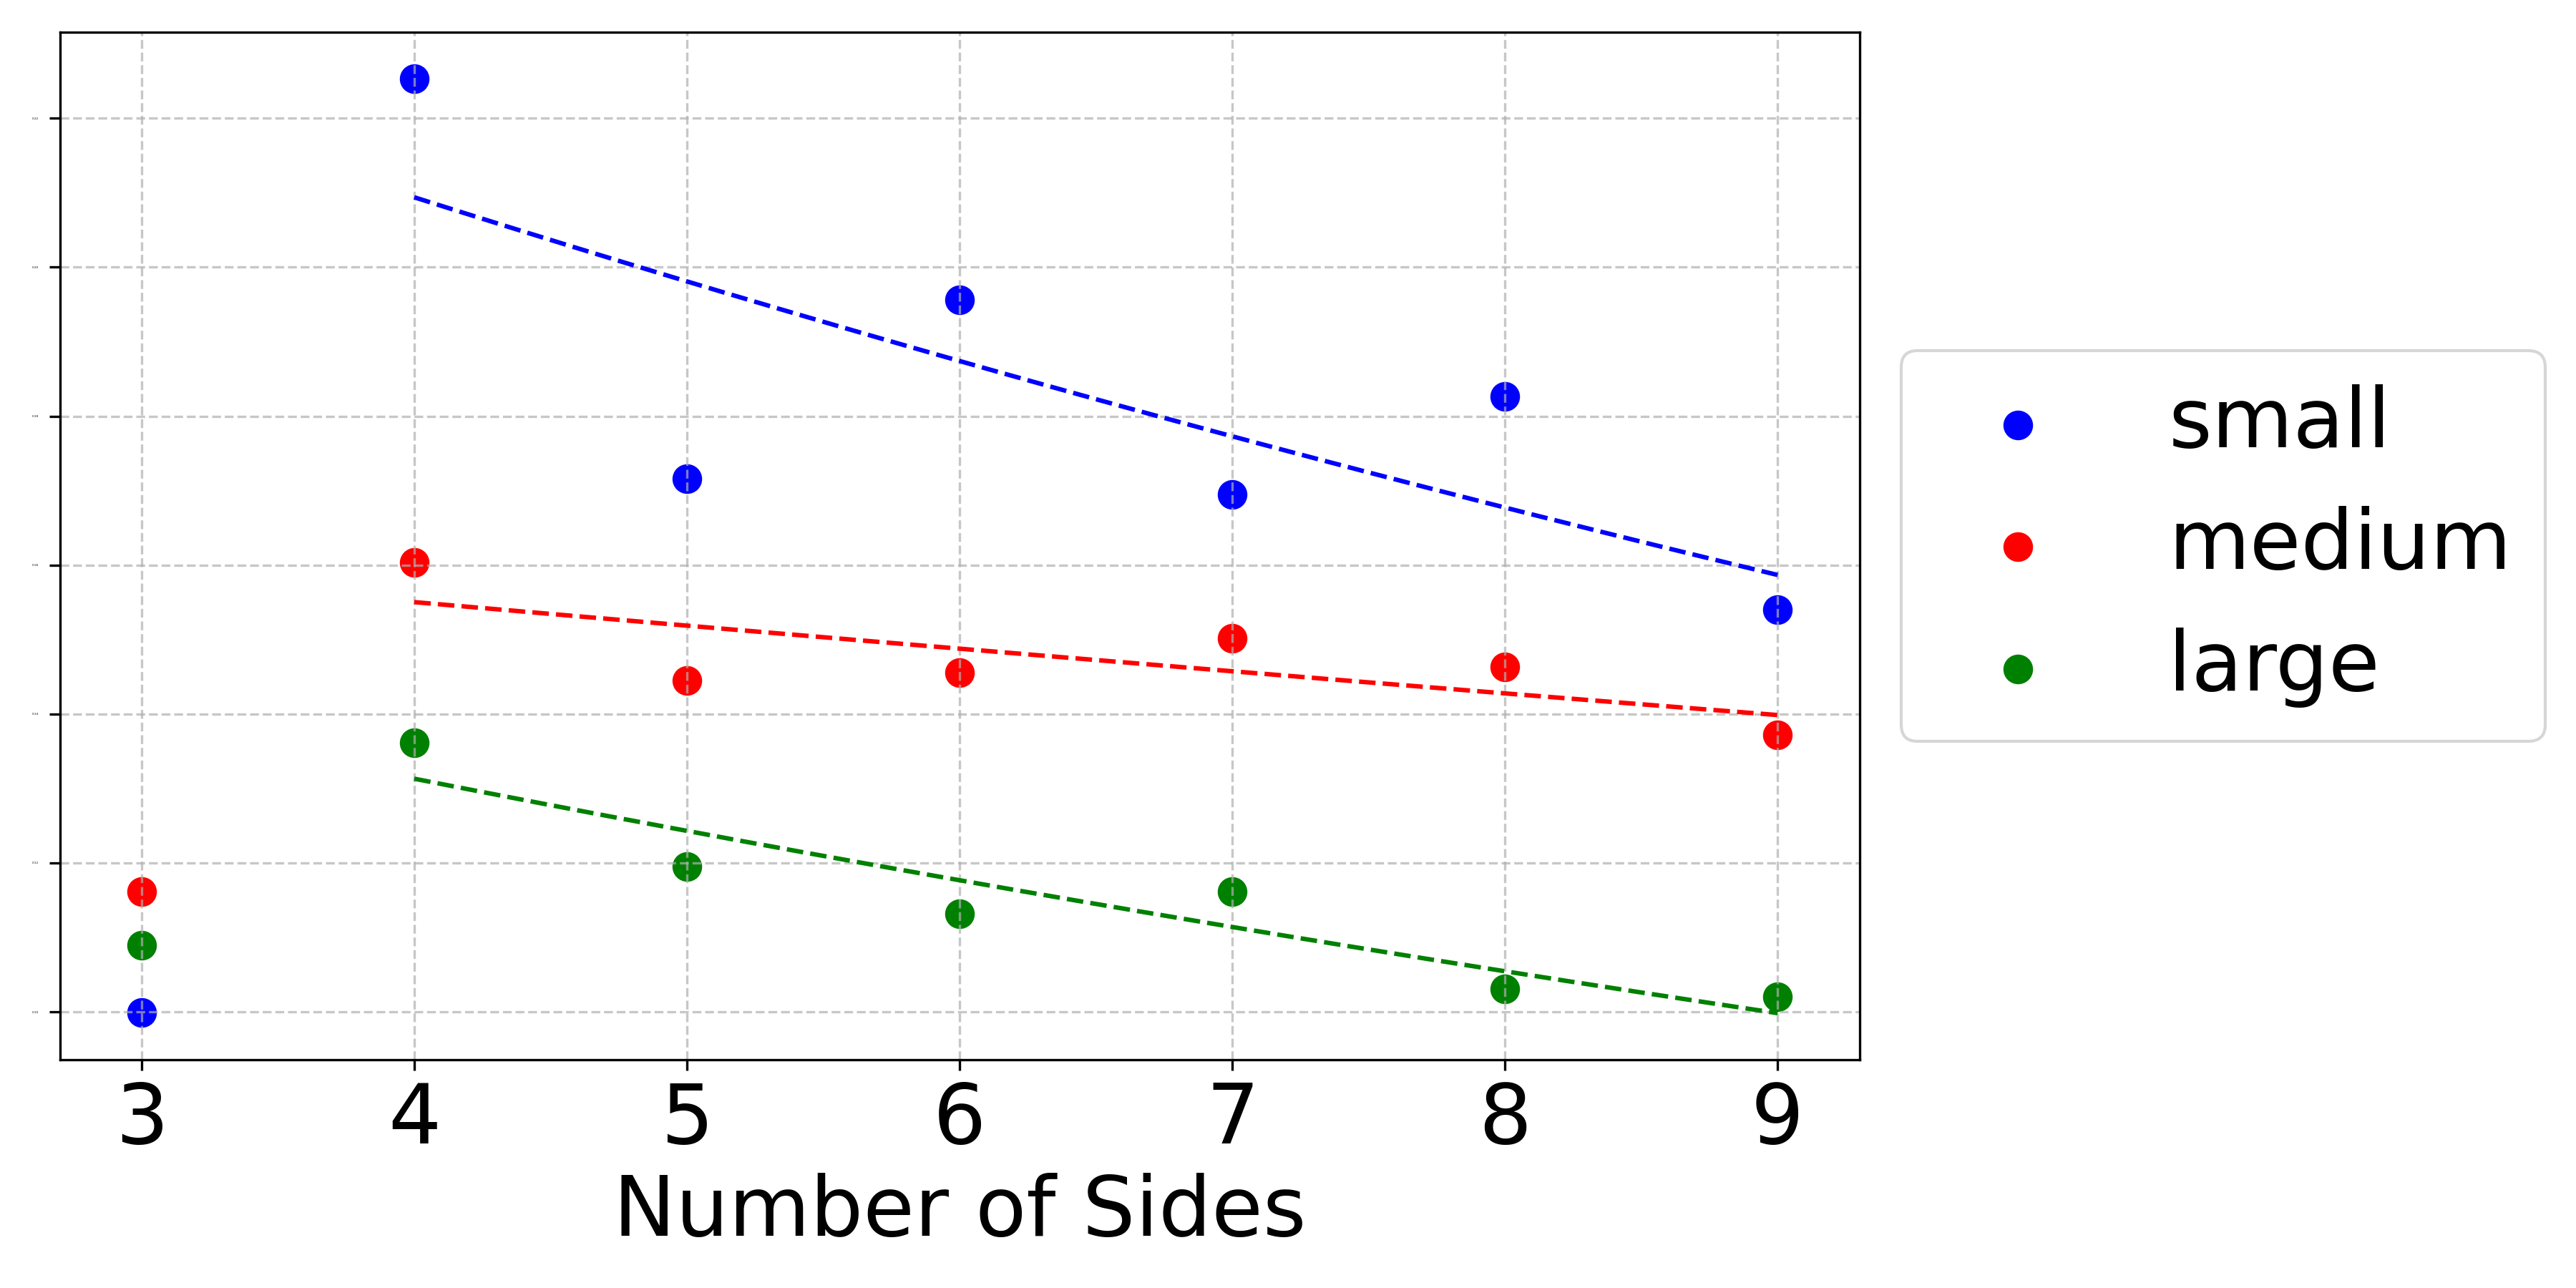
\includegraphics[width=1\columnwidth]{Images/Trend_total.png}
    \caption{Plotted curl by increasing number of sides in polygons, with correction for difference in area.}
    \label{fig:Trend}
\end{figure}
